\documentclass[a4paper, article, english, oneside, unknownkeysallowed, 12pt]{memoir} 
\usepackage{preamble}


\usepackage[
backend=biber,
style=authoryear-ibid,
maxcitenames=2, % show up to 2 authors in citations
mincitenames=1, % use "et al." if more than 2
maxbibnames=10, % show up to 10 names in bibliography
minbibnames=1,
uniquelist=false,
uniquename=false
]{biblatex}


\addbibresource{causal_effect_schools.bib}

\AtEveryBibitem{%
  \clearfield{urlyear}%
  \clearfield{urlmonth}%
  \clearfield{urlday}%
  \clearfield{urldate}%
}

% Name and Title
\title{Do High Schools Shape College Choices? Evidence from Centralized Assignment in Chile}
\author{ Bruno E. Aravena-Magüida}
\date{May 2026}

% Header (top) and footer (bottom)
\pagestyle{fancy}
\fancyhead[R]{\emph{Do High Schools Shape College Choices?}}
 \fancyhead[L]{BEAM} % keep section names
\fancyfoot[R]{}
\fancyfoot[L]{}


\begin{document}

% Prints title block from macros given above
\maketitle

\begin{abstract}
School quality is usually measured with test scores, but high schools may also shape students' college choices.
This paper studies this question in Chile, where centralized assignment creates lottery variation in high-school offers.
I link assignment records to administrative data on school enrollment, standardized achievement, and higher-education applications and enrollment.
I estimate observational school value added for math, language, STEM enrollment, and institutional quality, using a rich set of pre-treatment controls.
I then test whether lottery-induced attendance at higher-value-added schools improves the corresponding outcome, controlling for expected value added in each student's assignment portfolio.
Achievement pass-through estimates are 0.841 for math and 0.835 for language, close to benchmarks from settings with lagged test scores.
Higher-education value added also predicts causal changes in later choices: pass-through is 0.689 for STEM enrollment and 1.153 for institutional quality.
Heterogeneity estimates suggest that the pass-through of math value added varies substantially across the baseline math achievement distribution.
Although the correlation between estimated math and STEM value added is low (0.061), an orthogonal value-added exercise shows that causal effects on STEM enrollment are not explained by math value added.
High schools therefore shape college choices through dimensions of school value that achievement value added alone does not capture.
\end{abstract}

% Prints a table of contents
\setcounter{tocdepth}{2}
\renewcommand\contentsname{}
%\tableofcontents* 

\clearpage
\section{Introduction}

School quality is usually summarized by achievement.
This is natural: test scores are widely available, comparable across schools, and predictive of later outcomes.
But school and teacher effects are not necessarily one-dimensional.
Recent work shows that schools and teachers can affect attendance, behavior, crime, teenage motherhood, labor-market outcomes, and other long-run outcomes in ways that are only weakly related to test-score effects \parencite{jackson_what_2018, beuermann_what_2023, rose_effects_2022, angrist_methods_2023}.
Families and policymakers might therefore care about school quality measures that capture more than just achievement.

This broader view of school quality is especially relevant for high schools.
High schools are the last formal educational institutions students attend before making higher-education choices, and those choices are consequential.
Whether students enter higher education, which institutions they attend, and which fields they choose all matter because returns vary substantially across institutions and fields of study \parencite{kirkeboen_field_2016}.
Yet many measures of school effects on higher education are coarse, focusing on enrollment or persistence rather than on the type of institution or field students enter.

There are also good reasons to think that higher-education choices are shaped by frictions that schools may influence.
Prior work documents large differences in application and enrollment behavior across groups of students, and shows that relatively small interventions can change college search, application, and major choice \parencite{hoxby_what_2015, dynarski_closing_2021, hastings_informed_2016, chetty_diversifying_2025}.
If high schools differ in counseling, information provision, expectations, peer norms, academic confidence, or preparation for particular fields, then their effects on higher education may extend beyond their effects on achievement.

This paper asks whether high schools causally affect higher-education choices, and whether those effects are captured by traditional achievement value added.
The main empirical challenge arises from the fact that students and families sort across schools.
Families choose schools based on resources, preferences, networks, location, and expectations; these same characteristics may also shape later higher-education choices.
As a result, differences across schools may reflect both causal school effects and the underlying characteristics of the students and families who select into them.

I address this challenge using Chile's centralized school assignment system, the Sistema de Admisi\'on Escolar (SAE).
SAE assigns students to public and private-subsidized schools through a centralized mechanism that uses random tie-breakers when schools are oversubscribed.
The system covers a large national school sector, allowing me to study school effects at a scale that is unusual in lottery-based designs.
This assignment variation can be linked to administrative data covering school enrollment, standardized tests, and higher-education applications and enrollment.
Linking random assignment in the mechanism to higher-education choices allows me to answer this question in a national context.


The analysis proceeds in two steps.
First, I estimate observational value added for each school and outcome in the broad exam-taker panel.
These measures are school fixed effects from regressions that adjust for rich pre-treatment controls, including grade-4 standardized test scores, family-background variables, and middle-school controls.
Second, I use SAE lottery offers to ask whether schools that look better in observational value-added terms also produce larger causal effects, while controlling for expected value added in each student's assignment portfolio.


I summarize this relationship with a pass-through coefficient, $\theta$.
If $\theta=1$, then the causal effect induced by complying with a lottery offer equals the gain predicted by observational value added for that outcome.
If $\theta=0$, the observational value-added measure has no causal predictive content along the lottery-induced margin.
The main estimates suggest substantial pass-through.
For achievement, the estimates are 0.841 for math and 0.835 for language.
For higher-education outcomes, the pass-through is 0.689 for STEM enrollment and 1.153 for institutional quality.

In practical terms, schools that observationally look better at raising achievement or higher-education outcomes also tend to have causal effects on those same outcomes, though the causal effects are smaller than the observational differences.
The achievement estimates are close to comparable validation estimates in \textcite{angrist_leveraging_2017} despite the absence of immediately lagged outcomes.
This validates the rich set of pre-treatment controls used here, which can also be applied to outcomes, such as higher-education choices, for which lagged measures are unavailable.

I then ask for whom observational value-added measures are most informative.
Splitting the sample by baseline grade-4 math achievement shows that math value added is much more predictive for higher-achieving students, rising from 0.145 in the bottom quintile to 1.317 in the top quintile.
The language and higher-education value-added measures have more stable pass-through estimates across the baseline achievement distribution.
This result suggests that, at least for math achievement, students differ in how much they benefit from policies that provide information about school value added.


Finally, I examine whether STEM effects are simply achievement effects in another form.
To do this, I construct an orthogonal value-added measure that removes from STEM-enrollment value added the part predicted by math value added.
Math and STEM value added are already weakly related, and the IV results confirm that the orthogonal STEM component predicts STEM enrollment but not math achievement.
Conversely, math value added predicts math achievement but not STEM enrollment.
These results suggest that high schools differ along multiple dimensions, and that value added should not be treated as a single-dimensional measure of school quality.
In particular, they show that schools affect higher-education decisions, such as field choice, beyond their effects on achievement.

The paper contributes to three literatures.
First, it contributes to work on teacher and school value added.
A large literature estimates the effects of teachers and schools on test scores and longer-run outcomes \parencite{chetty_measuring_2014, dobbie_medium-term_2015, jackson_what_2018, beuermann_what_2023, rose_effects_2022}.
This work increasingly emphasizes that test-score value added may miss important dimensions of educational production.
I extend this idea to high-school effects on higher-education choices, where the relevant outcomes include field and institutional quality rather than only enrollment or achievement.

Second, the paper contributes to the literature using lotteries and centralized assignment systems to estimate school effects \parencite{abdulkadiroglu_elite_2014, abdulkadiroglu_research_2017, angrist_credible_2024}.
In the spirit of \textcite{angrist_leveraging_2017}, I ask whether observational value-added measures are useful guides to causal school effects.
The contribution here is to apply this pass-through logic to a national high-school assignment system and to outcomes observed after students transition into higher education.

Third, the paper contributes to work on higher-education choice.
Prior research shows that the field and institution students choose matter for later outcomes, and that information and application frictions can change those choices \parencite{kirkeboen_field_2016, hoxby_what_2015, dynarski_closing_2021, hastings_informed_2016, chetty_diversifying_2025}.
I study high schools as a possible upstream source of these differences.
Rather than evaluating a particular counseling or information intervention, the paper measures whether the high-school system itself generates causal differences in students' higher-education paths.

The rest of the paper is organized as follows.
Section 2 describes the Chilean setting and the linked administrative data.
Section 3 presents the empirical framework.
Section 4 reports the main results, heterogeneity by baseline achievement, and the orthogonal math/STEM value-added exercise.
Section 5 concludes.

\clearpage
\section{Context and Data}

\subsection{Institutional Setting}

Chile is a useful setting for this project because national administrative data record school enrollment, academic histories, standardized achievement, and higher-education choices with scrambled individual identifiers that allow students to be matched across systems.
Formal secondary education begins in grade 9 and lasts four years.
Students may attend public, private-subsidized, or private non-subsidized schools.
Public and private-subsidized schools are publicly financed and participate in the centralized school assignment system described below, while private non-subsidized schools remain outside that mechanism.
In the broad grade-8 universe used in the analysis, private non-subsidized schools account for about 9.3\% of students.
The lottery-based analysis is therefore drawn from the public and private-subsidized sector, with additional sample restrictions for timely SAE application and assignment risk described below.

\subsection{Student Panel and Baseline Controls}

I construct the broad analysis panel by merging annual enrollment, grade progression, attendance, grades, and completion records using the scrambled student identifier.
The panel starts from the universe of students first observed in grade 8 between 2017 and 2020, producing 944,360 students across four cohorts.
The main high-school exposure is observed for 4,133 RBDs.
I define high-school exposure as the school identifier (RBD) where a student spends the most time after grade 8.
This definition smooths over short enrollment spells and transfers, and it gives a single high-school measure for each student.
I define middle-school attendance analogously as the RBD where the student spends the most time in grades 5 to 8.
The same histories let me construct pre-treatment middle-school controls, including standardized measures of grades and attendance before high school.

Baseline achievement comes from SIMCE, Chile's national standardized assessment system.
SIMCE is administered in different grades depending on the year, including grades 4, 8, and 10.
Because the COVID-19 pandemic disrupted testing in 2020 and 2021, grade-8 and grade-10 measures are not available for all cohorts in the same way.
I therefore use grade-4 SIMCE as the main pre-treatment achievement control.
This gives a nationally comparable measure of math and language skills before high-school assignment for 771,968 students in the broad panel.

The SIMCE files also contain parent-survey information.
I use these surveys to measure family background before treatment, including household income, parental education, indigenous origin of the parents, and early-childhood attendance.
These variables are useful because they proxy for family resources and prior investments that may influence both high-school choices and later higher-education outcomes.
When parent-survey variables are missing, I use pre-treatment school and neighborhood cells to impute medians where enough donor observations are available; remaining missing values are left missing.

\begin{table}[H]
\centering
\caption{Main data sources and sample sizes}
\label{tab:data-samples}
\begin{tabular}{lr}
\toprule
Sample definition & Students \\
\midrule
Broad grade-8 universe, 2017--2020 & 944,360 \\
Plus grade-4 SIMCE math and language controls & 771,968 \\
Plus math or language admission-test outcome & 650,950 \\
\midrule
SAE lottery sample with assignment risk & 163,600 \\
Plus math or language admission-test outcome & 106,374 \\
\bottomrule
\end{tabular}
\end{table}

Table~\ref{tab:data-samples} summarizes how the linked administrative sources map into the two samples used in the analysis.
Rows within each panel should be read cumulatively.
The broad exam-taker panel is used to estimate the main school value-added measures, while the SAE lottery exam-taker sample is used to validate those measures using assignment variation.

\subsection{Centralized School Assignment}

Chile's centralized school assignment system, the Sistema de Admisi\'on Escolar (SAE), assigns students to participating schools through a version of student-proposing Deferred Acceptance.
Families submit ranked lists of schools.
The mechanism combines these rankings with school vacancies and priority rules, and it uses random tie-breakers when there are more applicants than seats within a priority group.
Conditional on the information that determines priorities and assignment probabilities, these tie-breakers generate the quasi-experimental variation used in the empirical design, following the centralized-assignment research design described by \textcite{abdulkadiroglu_research_2017}.

Implementing this design requires recovering each applicant's probability of assignment to each school in the submitted portfolio.
I do this by replicating the SAE assignment algorithm and repeatedly simulating counterfactual lottery draws.
As a diagnostic check, when I run the replicated algorithm using the original lottery numbers for the 2018--2021 regular grade-9 processes, I reproduce more than 99\% of observed first-round assignments in each of the four cohorts.
The remaining mismatch reflects institutional features that are difficult to fully recover from public documentation, but the high replication rate gives confidence that the simulated probabilities capture the relevant assignment risk.

I use applications to grade-9 vacancies to construct the lottery sample.
The estimation sample consists of timely SAE applicants, meaning students who apply in the assignment process corresponding to their grade-8 cohort, and who have assignment risk in the simulated data.
Assignment risk means that the simulated assignment probabilities do not place all probability mass on a single school.
This sample contains 163,600 students from the 2018--2020 cohorts.\footnote{The 2021 grade-8 cohort is omitted for data-availability reasons rather than design reasons.
At the time of writing in June 2026, the relevant public outcome files for that cohort had not yet been posted.
I expect to incorporate the cohort once those files are released, likely around July 2026.}
The main estimation sample further restricts to the 106,374 lottery-risk students with an observed math or language national admission-test score.
On average, these students have positive simulated assignment probability at about 3.1 schools; the median is 3 and the 90th percentile is 5.
About 86.5\% have an actual school RBD recorded as the first-round offer.
The remaining students have no school assigned in the first round of the offer file, and are retained with the offer instrument coded accordingly.
The first-round offered RBD is the source of lottery variation, while the student's realized high-school exposure is measured by the most-time RBD described above.

The value-added exercise uses the broader exam-taker panel, while the causal estimates use the smaller lottery-risk exam-taker sample.
This distinction is central to the interpretation.
The broad exam-taker panel improves precision in estimating school-level outcome gradients, and the lottery sample then tests whether those observational value-added measures have causal signal on the centralized-assignment margin.
The results therefore speak most directly to students and schools represented in the SAE lottery-risk sample.
Because SAE covers the public and private-subsidized sector, this is a large and policy-relevant part of the high-school market, but extrapolating to private non-subsidized schools or non-lottery margins requires assuming that the same value-added gradients are comparable there.

\subsection{Higher-Education Outcomes}

The higher-education system also generates administrative data on applications, admission scores, and enrollment.
Taking the national admission exam is a choice for secondary-school students, but it is the standard route into selective higher education.
Students who apply through the centralized admission system take mandatory math and verbal components, and may also take optional subject exams.\footnote{The national admission exam was called the PSU through 2020, the PTU in 2021--2022, and the PAES from 2023 onward.}
I use the mandatory math and language scores as achievement outcomes, standardizing them within test year to make them comparable across test regimes.

Higher-education applications and admissions are organized at the program-institution level.
A student's admission depends on entrance-exam scores, school GPA-based scores, ranked program preferences, and the weights each program assigns to score components.
This structure is useful because it makes higher-education choices much richer than a single college-enrollment indicator: students choose not only whether to enroll, but also which institution, program, and field to pursue.

I link the school panel to higher-education matricula records for first observed enrollment.
The main field-choice outcome is an indicator for enrollment in a STEM field, defined from the field classification of the first higher-education enrollment.
I focus on STEM because it is substantively important and closely connected to achievement, but the same data structure could be used to study other fields in future versions or appendix tables.
The main institutional-quality outcome is institutional accreditation years.
Institutional accreditation is a state-recognized quality certification process overseen by the National Accreditation Commission (CNA-Chile), and institutions can be accredited for up to seven years.
This is a crude measure of institutional quality, but it is observed in the matricula records and provides a simple way to distinguish higher- and lower-quality enrollment destinations.
Together, STEM enrollment and institutional accreditation years allow me to study whether high schools affect the type and quality of the higher-education paths students enter, not just whether students enter higher education at all.

Students without an observed higher-education enrollment are coded as zero for unconditional enrollment outcomes such as STEM enrollment.
For institutional-accreditation years, non-enrollment is also coded as zero, while observed enrollment records with missing accreditation inputs are left missing.
This zero-coding is an outcome definition rather than a missing-data imputation.
The main value-added and IV estimations restrict to students with an observed math or language national admission-test score.
Within this exam-taker sample, the zero-coded higher-education outcomes mainly distinguish students who take the admission exam and do or do not continue into the corresponding enrollment outcome.
In the broad panel, 650,950 students have a math or language admission-test outcome.
Among these exam takers, 536,240 have a first higher-education enrollment record and the unconditional STEM enrollment rate is 25.0\%.

\clearpage 
\section{Empirical Framework}

This section describes the empirical object and the research design.
The goal is not to estimate a separate causal effect for every school and every possible margin of substitution.
Instead, I ask whether an outcome-specific observational value-added measure is informative about causal effects generated by lottery-induced changes in school attendance.
The design therefore collapses school effects into scalar measures and estimates a pass-through coefficient for each outcome.

\subsection{School Effects and Observational Value Added}

I use a constant-effects value-added model as a guide:
\begin{equation}
  Y_i^m(j) = \mu^m + V_j^m + \epsilon_i^m,
  \label{eq:potential-va}
\end{equation}
Here, $Y_i^m(j)$ is student $i$'s potential outcome for outcome $m$ if assigned to high school $j$.
The index $m$ denotes the outcome, and $j$ denotes the high school.
The term $\mu^m$ is the average level of outcome $m$ under the student-weighted average school.
The term $V_j^m$ is the contribution of school $j$ to outcome $m$ relative to that average.
The term $\epsilon_i^m$ captures student-level determinants of outcome $m$ that do not vary with the assigned school in this constant-effects representation.
I normalize school effects so that their student-weighted mean is zero, $\sum_j \omega_j V_j^m = 0$, where $\omega_j$ is the share of students linked to school $j$ in the value-added sample.
This centering means that the weighted average of $V_j^m$ across schools is exactly zero.
A positive $V_j^m$ therefore denotes a school above the student-weighted average for outcome $m$, while a negative value denotes a school below that average.
The main outcomes are achievement in math and language, STEM enrollment, and institutional quality in higher education.

The first step constructs observational value added in the broad exam-taker panel.
For each outcome $m$, I estimate
\begin{equation}
  Y_i^m = \alpha^m + \lambda_{s(i)}^m + X_i'\Gamma^m + u_i^m,
  \label{eq:observational-va}
\end{equation}
where $s(i)$ is the student's main high-school RBD and $X_i$ contains pre-treatment controls.
These include cohort, gender, age, grade-4 SIMCE math and language, family-background measures from SIMCE parent surveys, and middle-school controls from grades 5 to 8.
I define the observational value-added measure $\widehat{V}_j^m$ as the centered empirical analogue of $V_j^m$: the estimated school fixed effect $\widehat{\lambda}_j^m$ from equation~\eqref{eq:observational-va}, centered using the same student-weighting convention.

Importantly, these fixed effects by themselves answer an observational question: conditional on $X_i$, which schools have higher average outcomes?
If school assignment in the broad panel were truly random, then the centered fixed effect $\widehat{\lambda}_j^m$ would identify $V_j^m$ up to sampling error.
In practice, students sort across schools, so the fixed effects may combine true school effects with any remaining selection not absorbed by controls.
The second step therefore asks whether the part of $\widehat{V}_j^m$ shifted by the SAE lotteries corresponds to causal effects in the same outcome.


\subsection{Assignment Risk and Expected Value Added}

SAE applicants submit rank-ordered lists of schools.
Let $Z_i$ denote the first-round school offer and $D_i$ denote the school attended, measured by the post-grade-8 most-time RBD.
A student has a preference and priority type $\theta_i$, and the assignment mechanism implies an assignment-probability vector $p_i=(p_{i1},...,p_{iJ})$, where $p_{ij}=Pr(Z_i=j)$.
Under equal treatment of equals, students with the same type have the same assignment probabilities \parencite{abdulkadiroglu_research_2017}.
For pre-treatment characteristics and potential outcomes fixed under re-randomization,
\begin{equation}
  (Y_i^m(1),...,Y_i^m(J), X_i) \ind Z_i \mid p_i.
  \label{eq:offer-independence}
\end{equation}

The raw vector $p_i$ is high-dimensional, because students can rank many different combinations of schools.
For an outcome-specific scalar value-added measure, I summarize assignment risk by the expected value added in the student's portfolio:
\begin{equation}
  E_i^m = \sum_j p_{ij}\widehat{V}_j^m.
  \label{eq:expected-va}
\end{equation}
This is the average value added the student would receive over repeated randomizations of the assignment mechanism, holding the submitted application and priorities fixed.
In the main IV specification, this scalar expected value replaces a large set of school-specific probability controls.

For each outcome $m$, define the value added of the attended school and offered school as
\begin{equation}
  A_i^m = \widehat{V}_{D_i}^m,
  \qquad
  O_i^m = \widehat{V}_{Z_i}^m.
  \label{eq:attended-offered-va}
\end{equation}
The instrument is $O_i^m$, the value added of the school generated by the lottery offer.
The endogenous variable is $A_i^m$, the value added of the school actually attended.
The notation is mnemonic: $O_i^m$ is the value added of the \textbf{O}ffered school, and $A_i^m$ is the value added of the \textbf{A}ttended school.
Because assignment offers vary randomly conditional on the assignment probabilities, variation in $O_i^m$ around $E_i^m$ provides quasi-experimental variation in the quality of the school offer.


\subsection{Pass-Through IV Specification}

The first empirical question is whether observational value added predicts causal effects on the same outcome.
Specifically, when the assignment mechanism moves a student toward a school with higher $\widehat{V}_j^m$, does outcome $m$ rise, and by how much relative to the observational difference encoded in $\widehat{V}_j^m$?
The main IV system is given by the following pair of equations:
\noindent
  \begin{equation}
    \begin{aligned}
      Y_i^m ={}& \alpha^m + \theta^m A_i^m + \rho^m E_i^m +  W_i'\delta^m + \eta_i^m,
    \end{aligned}
    \label{eq:pass-through}
  \end{equation}

  \begin{equation}
    \begin{aligned}
      A_i^m ={}& a^m + \kappa^m O_i^m + \rho_A^m E_i^m +  W_i'\delta_A^m + \nu_i^m.
    \end{aligned}
    \label{eq:first-stage}
  \end{equation}

Here, $Y_i^m$ is student $i$'s realized value of outcome $m$. We can see that the value-added of the attended school ($A_i^m$) is instrumented with the value added of the school offered through the assignment mechanism ($O_i^m$).
$E_i^m$ is the expected value added implied by the student's assignment-probability vector.
Finally, $W_i$ is a parsimonious lottery-sample control vector containing cohort, gender, age, and grade-4 SIMCE math and language.
This differs from the richer control vector used to construct $\widehat{V}_j^m$ in equation~\eqref{eq:observational-va}, which also includes family-background and middle-school controls.
The rich controls enter through the construction of the school value-added measures, while equation~\eqref{eq:pass-through} asks whether those pre-constructed measures pass through in the SAE lottery sample after conditioning on assignment risk and core baseline covariates.
All reported specifications use heteroskedasticity-robust standard errors.

The coefficient $\theta^m$ is the key object.
It measures how much of the observational value-added difference induced by the lottery offer passes through into causal effects on the same outcome.
If $\theta^m=1$, then a one-unit increase in observational value added causes a one-unit increase in the outcome.
If $\theta^m=0$, the observational measure has no causal predictive content along the lottery-induced margin.
Values between zero and one imply that observational value added is directionally informative, but overstates the causal effect of attending higher-value-added schools.

The scalar design is useful because a fully flexible school-specific IV design would be high-dimensional and would mix many margins of substitution across fallback schools \parencite{angrist_methods_2023, kirkeboen_field_2016}.
It instead asks whether movement toward schools with higher measured value added causes better outcomes, after controlling for the expected value added implied by each student's assignment risk.

A second empirical question is whether this pass-through relationship differs by students' baseline achievement.
To answer that question, I also estimate equation~\eqref{eq:pass-through} separately by quintiles of baseline grade-4 math achievement.
Because grade-4 SIMCE is measured before high-school assignment, these splits describe heterogeneity without conditioning on a post-treatment outcome.

\subsection{Orthogonal Value Added}

The final empirical question is whether higher-education value added is just achievement value added in another form.
In particular, I ask whether schools that raise STEM enrollment do so only because they raise math achievement, or whether they have a distinct STEM-related dimension.
To answer this, I construct two-dimensional value added for math achievement and STEM enrollment.
Let $\widehat{V}_j^{M}$ be math value added and $\widehat{V}_j^{S}$ be STEM-enrollment value added.
Following the EB-free variance-covariance logic in \textcite{rose_effects_2022}, I do not use empirical-Bayes posterior school effects for this exercise.
Instead, I estimate the projection coefficient using cross-cohort products of school-by-cohort residual means, which removes the mechanical same-cohort noise covariance from the math--STEM relationship.
I then residualize STEM value added on math value added:
\begin{equation}
  \widehat{V}_{j}^{S \perp M}
  =
  \widehat{V}_{j}^{S}
  -
  \widehat{\phi}\widehat{V}_{j}^{M}.
  \label{eq:orthogonal-va}
\end{equation}
Using this orthogonal component, I estimate a two-regressor IV model in which attended math value added and attended orthogonal STEM value added are both endogenous, and their offered analogues are the instruments.
For outcome $m \in \{M,S\}$:
\begin{equation}
  Y_i^m =
  \alpha^m
  + \theta_M^m A_i^M
  + \theta_{S\perp M}^m A_i^{S\perp M}
  + \rho_M^m E_i^M
  + \rho_{S\perp M}^m E_i^{S\perp M}
  + W_i'\delta^m
  + \eta_i^m.
  \label{eq:orthogonal-iv}
\end{equation}
This exercise follows the logic of orthogonal value-added measures used to distinguish achievement and non-achievement dimensions of educational production \parencite{jackson_what_2018, rose_effects_2022}.
In this setting, it tests whether schools with high STEM-enrollment value added are simply high math-value-added schools, or whether they have a distinct effect on students' higher-education field choices.

\clearpage 
\section{Results}

I organize the results in four blocks.
First, I describe the scale of the underlying outcomes and the distribution of the four observational school value-added measures.
Second, I report the main pass-through estimates for each outcome.
Third, I examine heterogeneity in pass-through by baseline grade-4 math achievement.
Finally, I use the two-dimensional value-added construction to separate math value added from the component of STEM value added that is orthogonal to math value added.

\subsection{Distribution of Value-Added Estimates}

Table~\ref{tab:school-va-distribution} reports the mean and standard deviation of each underlying student outcome alongside the student-weighted distribution of the corresponding school value-added measure.
The former capture variation across students; the latter capture estimated differences in school contributions.

\begin{table}[!htbp]
\centering
\begin{threeparttable}
\caption{Distribution of observational school value added}
\label{tab:school-va-distribution}
\small
\setlength{\tabcolsep}{3.5pt}
\begin{tabular}{lcc|cccccc}
\toprule
 & \multicolumn{2}{c|}{Outcome distribution} & \multicolumn{6}{c}{Value-added distribution} \\
\cmidrule(lr){2-3} \cmidrule(lr){4-9}
Outcome & \shortstack{Sample\\Mean} & \shortstack{Sample\\SD} & VA SD & P10 & P25 & P50 & P75 & P90 \\
\midrule
Math & 0.043 & 1.002 & 0.258 & -0.216 & -0.155 & -0.074 & 0.058 & 0.328 \\
Language & 0.049 & 0.989 & 0.188 & -0.202 & -0.135 & -0.030 & 0.095 & 0.238 \\
STEM enrollment & 0.252 & 0.434 & 0.078 & -0.078 & -0.045 & -0.012 & 0.031 & 0.086 \\
Institutional quality & 4.678 & 2.379 & 0.375 & -0.458 & -0.214 & -0.003 & 0.231 & 0.459 \\
\bottomrule
\end{tabular}
\begin{tablenotes}[flushleft]
\footnotesize
\item Notes: The table reports the student-weighted distribution of All-sample adjusted school value added. Schools are weighted by the number of students used to estimate the corresponding value-added measure. Sample Mean and Sample SD refer to the underlying outcome in the outcome-specific value-added regression sample; the remaining columns describe the value-added distribution. Math and language are measured in admission-test standard deviations, STEM enrollment in probability units, and institutional quality in accreditation years.
\end{tablenotes}
\end{threeparttable}
\end{table}


The achievement outcomes are standardized measures, so their sample means are close to zero and their standard deviations are close to one.
The mean STEM enrollment rate is 0.252, with a student-level standard deviation of 0.434, while institutional quality averages 4.678 accreditation years, with a standard deviation of 2.379 years.

The school value-added measures also display substantial dispersion.
The standard deviation of math value added is 0.258, and the gap between the 90th and 10th percentiles is 0.544 standard deviations.
For language, the corresponding standard deviation is 0.188 and the 90--10 gap is 0.440 standard deviations.
Among the higher-education outcomes, the standard deviation of STEM-enrollment value added is 0.078, or 7.8 percentage points, and its 90--10 gap is 0.164.
Institutional-quality value added has a standard deviation of 0.375 years and a 90--10 gap of 0.917 years.
These distributions show that the observational measures contain economically meaningful variation and provide the scale needed to interpret the pass-through estimates below.

\subsection{IV Pass-through Estimates}


Table~\ref{tab:main-four-va-results} reports the main IV estimates.
Each column uses the same outcome to construct the observational school value-added measure, the lottery-induced expected value-added instrument, and the realized attended school value-added treatment.
The coefficients can therefore be read as pass-through estimates: how much a lottery-induced increase in a school's observational value added translates into a causal gain in the corresponding student outcome.

The achievement estimates are close to one.
A one standard deviation increase in school math value added raises math achievement by 0.841 standard deviations, while the analogous estimate for language is 0.835.
The higher-education estimates are also positive.
The estimated pass-through is 0.689 for STEM enrollment and 1.153 for institutional quality, measured using institutional accreditation years.
Taken together, the estimates suggest that the observational school value-added measures are informative not only about test score production, but also about later higher-education choices.
They also provide reduced-form evidence that high schools causally affect all four outcomes studied here.
Lottery-induced movement toward schools with higher observational value added raises math achievement, language achievement, STEM enrollment, and institutional quality.
For STEM enrollment, this table does not yet show whether the effect operates through math achievement or through a distinct school dimension.
It does show, however, that the school assignment margin shifts later higher-education choices, not only test scores.

\begin{table}[!htbp]
\centering
\caption{Main scalar school-value IV estimates}
\label{tab:main-four-va-results}
\begin{tabular}{lcccc}
\toprule
 & \multicolumn{2}{c}{Achievement} & \multicolumn{2}{c}{Higher education} \\
\cmidrule(lr){2-3} \cmidrule(lr){4-5}
 & Math & Language & STEM enrollment & Institution quality \\
\midrule
$\theta$ & 0.841 & 0.835 & 0.674 & 0.680 \\
SE & (0.071) & (0.082) & (0.065) & (0.095) \\
Observations & 90,906 & 92,472 & 135,898 & 135,898 \\
\bottomrule
\end{tabular}
\end{table}



\subsection{Heterogeneity by Baseline Achievement}

Figure~\ref{fig:simce4-math-quintile-four-metrics} repeats the same four estimates separately by quintiles of baseline grade-4 math achievement.
This comparison is useful because it keeps the heterogeneity split pre-treatment and available for the full exam-taker analysis sample.
Table~\ref{tab:simce4-math-quintile-contrasts-q3} formally tests each quintile coefficient against the middle quintile, reporting $\widehat{\theta}_{Q_q}-\widehat{\theta}_{Q_3}$ for $q\in\{1,2,4,5\}$.

The clearest heterogeneity appears in math.
The bottom-quintile estimate is 0.145, compared with 0.940 in the middle quintile, a difference of $-0.795$ ($p<0.01$).
The top-quintile estimate is 1.317, or 0.377 above the middle quintile, although this difference is significant only at the 10 percent level ($p=0.093$).
The math estimates for the second and fourth quintiles are not statistically different from the middle-quintile estimate.

For language, none of the four contrasts with the middle quintile is statistically significant.
STEM-enrollment pass-through is lower in the second quintile by 0.469 ($p=0.026$) and lower in the fourth quintile by 0.388, with the latter difference significant at the 10 percent level ($p=0.085$).
The first- and fifth-quintile STEM estimates do not differ significantly from the middle-quintile estimate.
Institutional-quality pass-through is positive in every quintile, and none of its contrasts with the middle quintile is statistically significant.
Thus, the formal tests support meaningful heterogeneity in selected math and STEM contrasts, but not a uniform monotonic gradient across the baseline achievement distribution.

\begin{figure}[!htbp]
\centering
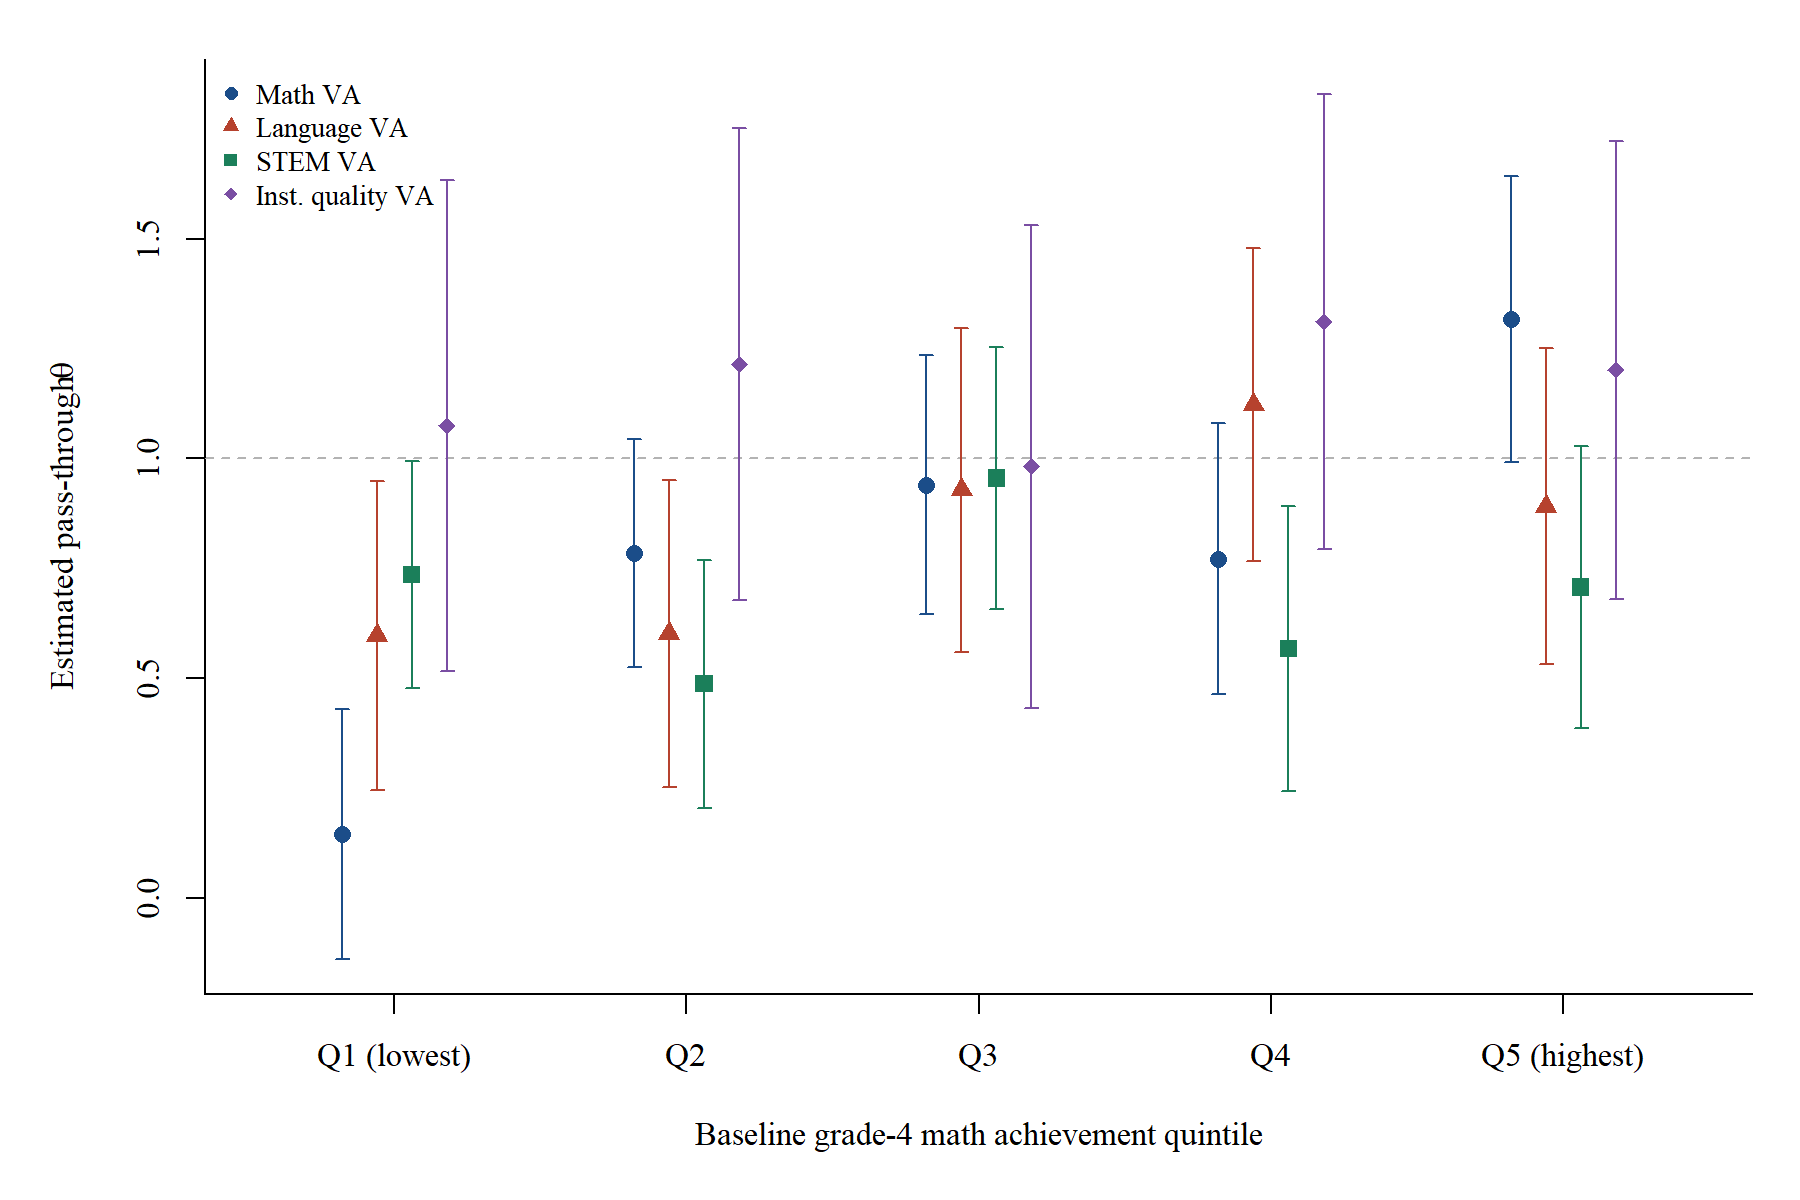
\includegraphics[width=.9\textwidth]{../../output/figures/results_section/simce4_math_quintile_four_metrics.png}
\caption{Scalar school-value IV estimates by baseline grade-4 math achievement quintile}
\label{fig:simce4-math-quintile-four-metrics}
\end{figure}
\begin{table}[!htbp]
\centering
\begin{threeparttable}
\caption{Differences in pass-through relative to the middle quintile}
\label{tab:simce4-math-quintile-contrasts-q3}
\small
\begin{tabular}{lcccc}
\toprule
Comparison & Math & Language & STEM enrollment & Institutional quality \\
\midrule
$Q1-Q3$ & -0.795*** & -0.332 & -0.220 & 0.093 \\
 & (0.209) & (0.260) & (0.202) & (0.400) \\
$Q2-Q3$ & -0.155 & -0.328 & -0.469** & 0.233 \\
 & (0.201) & (0.259) & (0.210) & (0.392) \\
$Q4-Q3$ & -0.169 & 0.193 & -0.388* & 0.330 \\
 & (0.218) & (0.262) & (0.225) & (0.386) \\
$Q5-Q3$ & 0.377* & -0.038 & -0.248 & 0.220 \\
 & (0.224) & (0.263) & (0.224) & (0.387) \\
\bottomrule
\end{tabular}
\begin{tablenotes}[flushleft]
\footnotesize
\item Notes: Each entry reports $\widehat{\theta}_{Q_q} - \widehat{\theta}_{Q3}$ for the indicated baseline grade-4 math achievement quintile. Heteroskedasticity-robust standard errors are reported in parentheses. Because quintile samples are disjoint, the contrast variance is the sum of the two coefficient variances. $^{*}p<0.10$, $^{**}p<0.05$, $^{***}p<0.01$.
\end{tablenotes}
\end{threeparttable}
\end{table}

\FloatBarrier

\subsection{Orthogonal Math and STEM Value Added}

The scalar estimates above treat each outcome-specific value-added measure one at a time.
I also construct a two-dimensional measure that separates math value added from STEM-enrollment value added.
Figure~\ref{fig:va-correlation-panels}, panel (a), first compares math and verbal value added as an achievement benchmark.
The two achievement measures are strongly related across schools, with a correlation of 0.645.
Panel (b) then compares math value added with STEM-enrollment value added.
In contrast to the two achievement measures, the school-level relationship between math and STEM value added is close to zero, with a correlation of 0.061.
This makes it possible to ask whether schools that improve STEM enrollment are doing so only because they are also high math value-added schools, or whether there is a distinct STEM-related component.

\begin{figure}[!htbp]
\centering
\subbottom[Math and verbal value added\label{fig:math-verbal-va-correlation}]{%
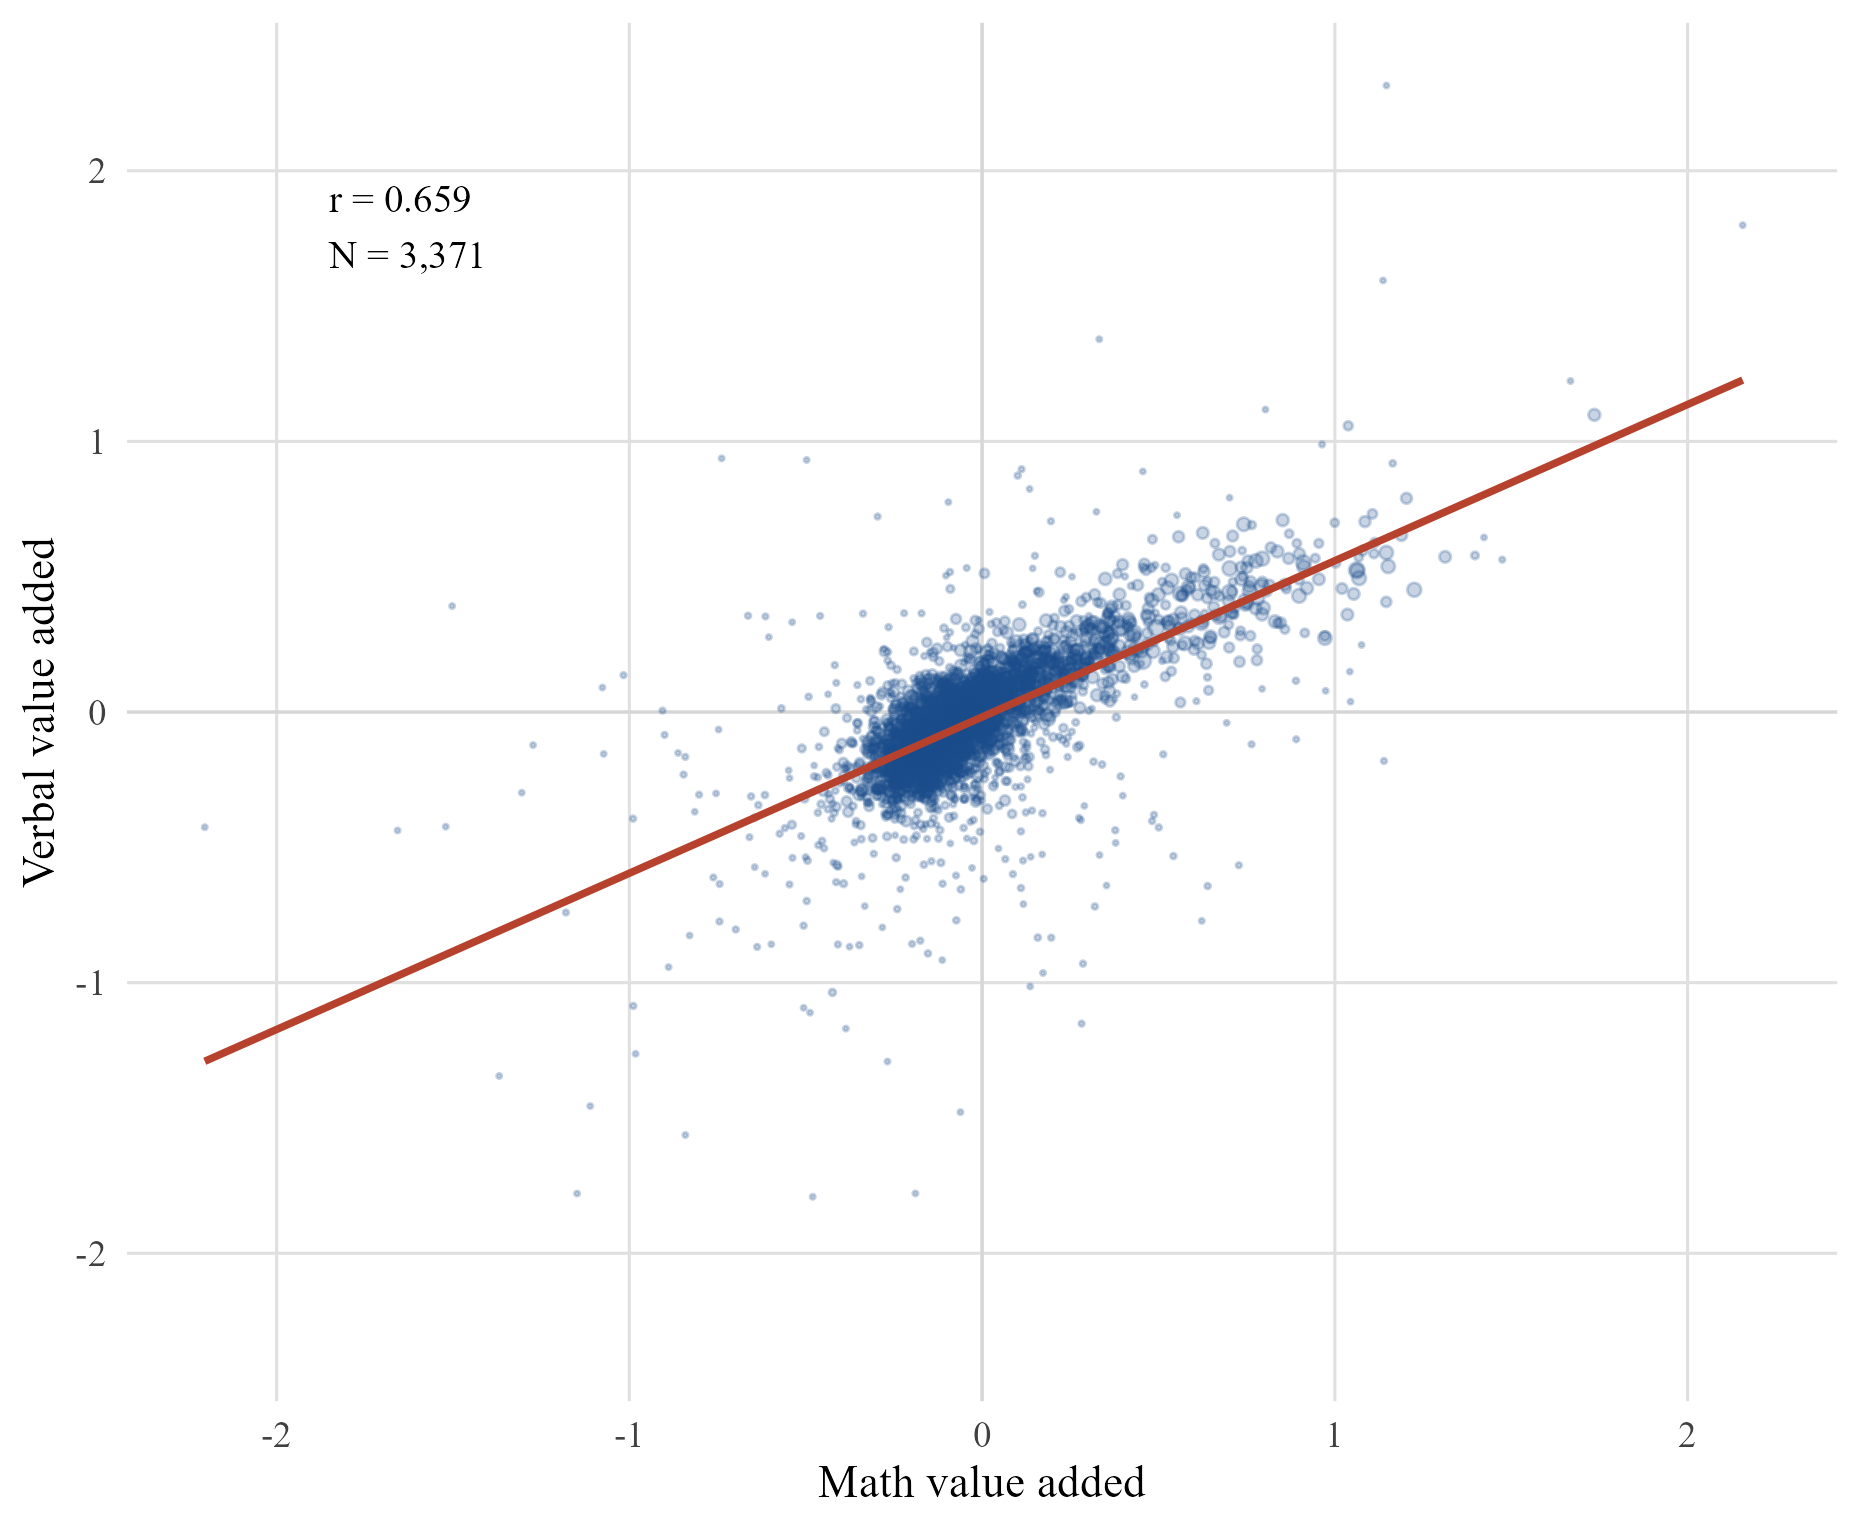
\includegraphics[width=.48\textwidth]{../../output/figures/results_section/math_language_va_correlation.png}%
}
\hfill
\subbottom[Math and STEM enrollment value added\label{fig:math-stem-va-correlation}]{%
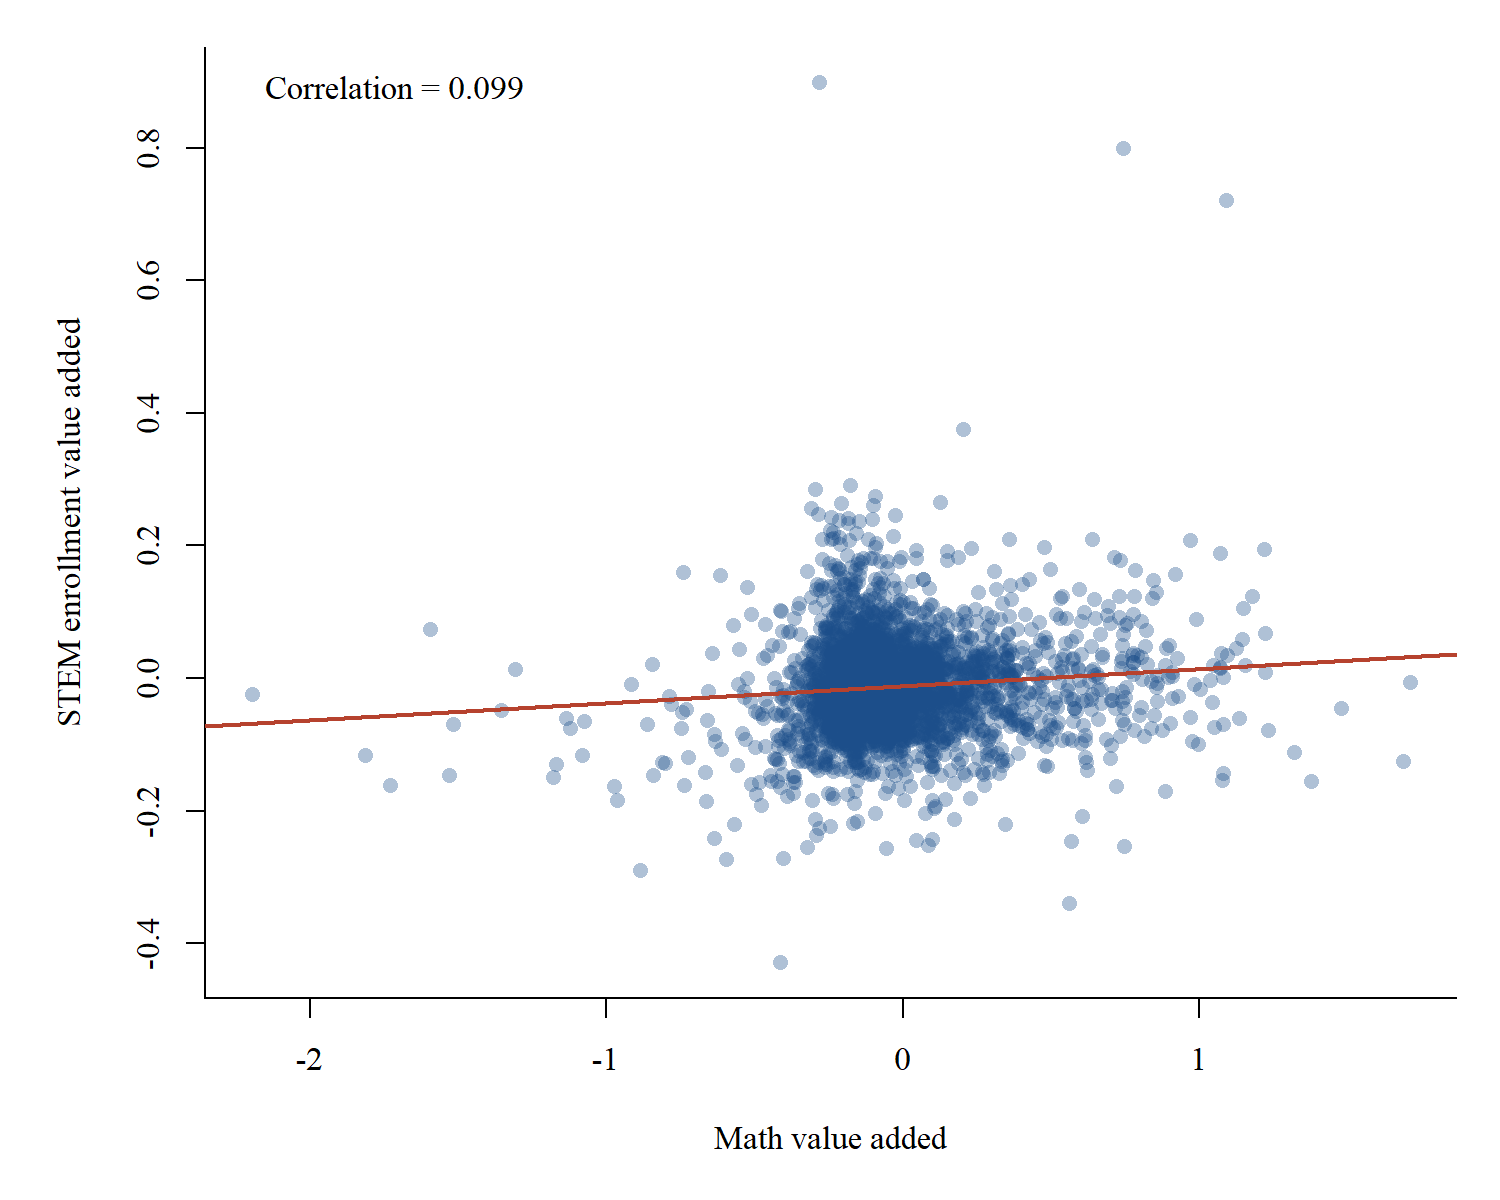
\includegraphics[width=.48\textwidth]{../../output/figures/results_section/math_stem_va_correlation.png}%
}
\caption{Relationships between math, verbal, and STEM observational value added}
\label{fig:va-correlation-panels}
\end{figure}
\FloatBarrier

Table~\ref{tab:orthogonal_school_va_iv_2x2} reports the corresponding two-regressor IV estimates where each column estimating equation \ref{eq:orthogonal-iv} on the corresponding outcome. 
Math value added strongly predicts math achievement, with an estimate of 0.847, but it does not predict STEM enrollment once the orthogonal STEM component is included.
Conversely, the STEM component orthogonalized against math value added strongly predicts STEM enrollment, with an estimate of 0.678, while it has essentially no relationship with math achievement.
The punchline is that STEM value added is not simply math value added translated into a higher-education outcome.
In the sense measured here, the STEM effects are not mediated through math value added.
Schools that move students into STEM do so along a dimension that is orthogonal to their math-achievement value added.
The estimates therefore point to different dimensions of school value that can be related to one another, but are not reducible to a single achievement index.
This uncovers a distinct dimension of school value added that matters for students' higher-education field choices.

\begin{table}[!htbp]
\centering
\caption{Two-dimensional orthogonal school-value IV estimates}
\label{tab:orthogonal_school_va_iv_2x2}
\begin{tabular}{lcc}
\toprule
 & Math score & STEM enrollment \\
\midrule
Math VA & 0.844 & -0.058 \\
 & (0.072) & (0.039) \\
STEM VA orthogonal to math & 0.017 & 0.656 \\
 & (0.111) & (0.066) \\
\bottomrule
\end{tabular}
\end{table}


\FloatBarrier

\clearpage 
\section{Conclusion}

This paper studies whether high schools affect higher-education choices in ways that are captured by, or distinct from, traditional achievement value added.
Using Chile's centralized school assignment system and linked administrative data, I first estimate observational school value added in a broad national panel and then use SAE lottery offers to test whether those measures predict causal effects.

The results suggest that the value-added measures constructed for new higher-education outcomes contain meaningful causal signal.
Achievement value added provides a useful benchmark: the pass-through estimates are 0.841 for math and 0.835 for language.
These estimates are somewhat below the unit benchmark, but they are close to comparable achievement-validity estimates in \textcite{angrist_leveraging_2017}, where lagged-score forecast coefficients are 0.864 for sixth-grade lotteries and 0.880 for all middle-school grades.
The similarity is reassuring because the present setting differs in two important ways.
First, the analysis is national in scope and covers a large, heterogeneous set of high schools rather than a narrower local market.
Second, and more importantly, I do not condition on a lagged version of the outcome.
This is a limitation for achievement, but it is also a deliberate feature of the design: the same value-added control set can be used for outcomes such as STEM enrollment and institutional quality, for which there is no natural lagged outcome before high school.
The close achievement benchmark therefore suggests that the value-added control set is strong enough to recover useful school value added even without a lagged outcome.
This makes the positive higher-education estimates more credible: value added for STEM enrollment and institutional quality predicts lottery-induced changes in those outcomes, with pass-through estimates of 0.689 and 1.153, respectively.

The heterogeneity results provide a separate lesson.
They suggest that value-added metrics need not be equally informative for every student group.
For math, the pass-through estimate rises from 0.145 in the bottom baseline-achievement quintile to 1.317 in the top quintile.
This gradient is hard to reconcile with a strict constant-effects interpretation, and it suggests that value-added validation exercises can be used to study heterogeneity itself.
At the same time, the STEM and institutional-quality estimates remain positive across baseline-achievement quintiles and show less of a monotone achievement gradient.
Taken at face value, this contrast is informative: heterogeneity may be substantial for some value-added dimensions but muted for others, and different baseline variables may reveal different gradients.

The orthogonal-value-added result speaks to a different and central question: are the STEM effects just achievement effects in another form?
The answer appears to be no.
The weak school-level correlation between math value added and STEM value added already suggests that these are not the same object.
More powerfully, the two-dimensional IV estimates show that math value added predicts math achievement but not STEM enrollment, while the STEM component orthogonal to math value added predicts STEM enrollment but not math achievement.
This leaves little evidence that the STEM enrollment effect is mediated through the math value-added dimension measured here.
Instead, the results point to multiple channels through which high schools shape later choices.
One channel is achievement production, which is visible in the math and language results and has been the focus of much of the value-added literature.
Another channel affects higher-education field choices in a way that is not reducible to test-score value added.
That distinction is the central punchline of the paper: high schools shape college choices, and STEM value added captures a dimension of school value that achievement value added misses.

For families and policymakers, the results imply that school quality information based only on achievement is incomplete.
Test-score value added is clearly informative, but it does not exhaust the ways in which high schools shape educational paths.
A deeper view of school quality should recognize that schools may affect both academic production and the later choices students make about fields and institutions.
This connects to evidence that school output is multidimensional and that families may or may not fully value the causal dimensions of school effectiveness when choosing schools \parencite{beuermann_what_2023, abdulkadiroglu_parents_2020, hastings_preferences_2007}.
The next question is whether families already anticipate these less visible dimensions of school value, or whether they would respond to information about them if it were made available.
Now that the paper shows that STEM-oriented school value added exists, the natural next step is to understand whether families internalize it ex ante, how it is produced inside schools, and whether information about it would change school choices.

\clearpage
\printbibliography
\end{document}
